\scanpage{19}
\mspage{- 3 -}
\figure{
\begin{tikzpicture}[x=1mm,y=1mm]
\fill (0,0)--(.6,1.3)--(.7,3)--(3.4,1.8)--(7.6,.6)--(7.5,-.4)--(3.4,.1)--cycle;
\end{tikzpicture}}

so that
\[
\begin{aligned}
(\unsure{P|p}_1,P_1)\circ\unsure{\Pi_0|\pi_0|\Pi_o|\pi_o}&=P_1\\
(P_1,P_2)\circ\Pi_0&=P_2\\
(P_2,P_1)\circ\Pi_0&=P_2\\
(P_2,P_2)\circ\Pi_0&=P_2.
\end{aligned}
\]

It is easy to check that $P_1:A\otimes A\longrightarrow k$ is a counit, that $\Pi_0$ is co-associative, co-commutative.
\margin{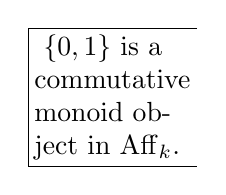
\begin{tikzpicture}[baseline=(note.base)]
\node[anchor=north west,align=left,text width=1.99cm,inner sep=2pt] (note) at (0,0)
{$\therefore\ \{0,1\}$ is a commutative monoid object in $\mathrm{Aff}_k$.};
\draw (note.north east)--(note.north west)--(note.south west)--(note.south east);
\end{tikzpicture}}

But $\{0,1\}(k)$ can't be a group object in sets.
\[
\begin{aligned}
&\text{\rq\rq}\\[-2pt]
&\{P_1,P_2\}.
\end{aligned}
\]

Moreover $A$ can't be given a co-inversion or antipodal map. One way of characterizing the inverse \inserted{$\sigma$} for \unsure{commut|commut.} gps is that $\exists\,\sigma:G\longrightarrow G$ \unsure{sud|such} that
\diagram{\begin{minipage}[t]{.47\linewidth}\vspace{0pt}\centering
\begin{tikzcd}[ampersand replacement=\&,row sep=large,column sep=small]
G\arrow[r,"{\unsure{I_G|1_G}\times\sigma}"] \&
G\times G\arrow[d,"\Pi","{\unsure{\cdot}}"{pos=.92,swap},"{\unsure{\cdot}}"{pos=.94}]\\
\& G
\end{tikzcd}
\end{minipage}\hfill
\begin{minipage}[t]{.48\linewidth}\vspace{0pt}
factors through the final then initial object :
\end{minipage}}
\diagram{\begin{tikzcd}[ampersand replacement=\&,row sep=2pt,column sep=3pt]
G\arrow[rr,"{I_G\times\sigma}"]\arrow[ddd] \& \& G\times G\arrow[ddd,"\Pi"] \& \&
 \text{i.e. that\unsure{.}}\arrow[dl,bend left=15]\\
\& {x\longmapsto(x,x^{-1})}\arrow[d,maps to] \& \& \vphantom{G} \&
 \begin{gathered}\text{commutes since}\\\text{the final }+\text{ initial}\\\text{objs coincide.}\end{gathered}\\
\& e.\& \& \&\\
e\arrow[rr,"{\unsure{\cdot}}"{pos=.94,below}] \& \& G \& \&
\end{tikzcd}}
% archive sheet number: 18
\clearpage
